%%% PREAMBLE - Do not touch %%%%%%%%%%%%%%%%%%%%%%%%%%%%%%%%%%%%%%%%%%%%%%%%%%%%%%
\documentclass[10pt,twocolumn,letterpaper]{article}
\usepackage[utf8]{inputenc}
\usepackage[brazil]{babel}
\usepackage{bm}
\usepackage{model}
\usepackage{times}
\usepackage{epsfig}
\usepackage{graphicx}
\usepackage{amsmath}
\usepackage{amssymb}
\usepackage{color}
\usepackage[pagebackref=true,breaklinks=true,letterpaper=true,colorlinks,bookmarks=false]{hyperref}

\cvprfinalcopy % *** Uncomment this line for the final submission
\def\httilde{\mbox{\tt\raisebox{-.5ex}{\symbol{126}}}}
\ifcvprfinal\pagestyle{empty}\fi

%%% Report beginning %%%%%%%%%%%%%%%%%%%%%%%%%%%%%%%%%%%%%%%%%%%%%%%%%%%%%%%%%%%%%%
\begin{document}

%%% Title and authors %%%%%%%%%%%%%%%%%%%%%%%%%%%%%%%%%%%%%%%%%%%%%%%%%%%%%%%%%%%%
\title {Predizendo o modelo da câmera de uma fotografia a partir de técnicas de aprendizado de máquina}
\author{Gustavo Ciotto Pinton, RA117136\thanks{Is with the Institute of Computing, University of Campinas (Unicamp). \textbf{Contact}: \tt\small{gustavociotto@gmail.com}}}

%%% Abstract %%%%%%%%%%%%%%%%%%%%%%%%%%%%%%%%%%%%%%%%%%%%%%%%%%%%%%%%%%%%%%%%%%%%%
\maketitle
\begin{abstract}
São propostos neste documento dois métodos de classificação baseados em aprendizado de máquina e capazes de determinar, a partir de uma foto, o modelo da câmera que a gerou. No total, 10 modelos de câmeras distintas, mas de mesmos fabricantes, são utilizados neste problema. O primeiro, baseado na técnica de regressão logística, consiste em separar as 10 classes em grupos binários de maneira a testar sempre um dos modelos contra os demais, enquanto que o segundo, baseado em redes neurais, busca diretamente a classe de determinada imagem, sem quaisquer divisão binária dos grupos. Além disso, neste artigo, estão descritos os atributos recuperados das imagens e os parâmetros configurados em cada um dos métodos, bem como a sua influência no resultado final. Por fim, são apresentados os resultados de cada uma das técnica e o score obtido para o problema na plataforma Kaggle.
\end{abstract}

%%% Introduction %%%%%%%%%%%%%%%%%%%%%%%%%%%%%%%%%%%%%%%%%%%%%%%%%%%%%%%%%%%%%%%%%
\section{Introdução}
\label{intro}

A técnica de regressão logistíca, ao contrário do método de regressão linear cujo objetivo é adequar os dados a uma equação linear, busca classificar os dados de entrada em dois grupos discretos, comumente denominados \(0\) e \(1\). Para tal, define-se a matriz \(\bm{x}\) de dimensões \(N + 1 \times M\)  contendo \(M\) entradas descritas por \(N + 1\) atributos (contando evidentemente um elemento de \textit{bias}), o vetor \(\bm{\theta}\) representando o peso que cada atributo terá no modelo e a uma função \(g\left(\bm{\theta}, \bm{x}^{(i)}\right)\) cujo conjunto imagem é o intervalo \([0,1]\). Esta última é responsável por predizer a classe \(\bm{\hat{y}}^{(i)}\) de cada entrada \(\bm{x}^{(i)}\), tendo em vista que valores \(\bm{\hat{y}}^{(i)}\) mais próximos de 0 indicarão que determinada entrada tem mais chance de pertencer à classe 0 e vice-versa. A função \(g\), a princípio, pode assumir qualquer equação desde que sua imagem fique entre 0 e 1. Para este documento, tal função assumirá a forma sigmoidal, conforme equação \ref{eq:sig}.

\begin{equation}
\label {eq:sig}
\bm{\hat{y}}^{(i)} = g \left(\bm{\theta},\bm{x}^{(i)}\right) = \frac {1}{1 + e^{-\bm{\theta}^T\bm{x}^{(i)}}}
\end{equation}

Neste caso, se \(\theta^T\bm{x}^{(i)}\) é grande, então \(e^{-\theta^T\bm{x}^{(i)}}\) tende a zero e a classe atribuida à entrada \(i\) será 1. Em oposição, se \(\theta^T\bm{x}^{(i)}\) é muito negativo, a função tenderá a 0, assim como a classe escolhida.

Assim como quase toda técnica de aprendizado de máquina, a determinação dos valores do vetor \(\bm{\theta}\) envolve a minimização de uma função de custo \(J(\bm{\theta}, \bm{x})\), descrita pela equação \ref{eq:cost}, a partir de um conjunto de entradas \(\bm{x}^{(i)}\) de saídas \(\bm{y}^{(i)}\) conhecidas.

\begin{equation}
\begin{split}
\label {eq:cost}
J(\bm{\theta}, \bm{x}) = -\frac{1}{M} \displaystyle\sum_{i=1}^{M} & \left[ \bm{y}^{(i)}\log \left( \bm{\hat{y}}^{(i)} \right) + \ldots \right. \\
& \left.  + \left(1 -\bm{y}^{(i)}\right)\log \left(1 - \bm{\hat{y}}^{(i)} \right) \right] \\
\end{split}
\end{equation}

Como visto em aula, a função \(J(\bm{\theta}, \bm{x})\) é convexa e, portanto, não possui mínimos locais além do global e sua minimização pode ser realizada também através do método de \textit {gradient descent}, explorada na última atividade. Os dados utilizados para a minimização \(\bm{x}^{(i)}\) e \(\bm{y}^{(i)}\) pertencem a um conjunto denominado \textbf{conjunto de treinamento}, enquanto que a validação dos parâmetros obtidos ocorre em um conjunto que recebe este mesmo nome. Um regra geral é separar 80\% dos dados disponíveis para treinamento e o restante, 20\%, para testes e validação.

Derivando-se parcialmente a equação \ref{eq:cost} em relação a \(\bm{\theta}_j\), obtém-se o coeficiente linear e portanto a direção que devemos tomar para nos aproximar do mínimo global. Repetindo o raciocínio para todos os parâmetros \(\bm{\theta}_j\), obtém-se à operação \ref{gd} que deve ser aplicada a cada um deles a cada iteração. Observa-se que, apesar de que o cálculo de \ref {eq:sig} ser totalmente diferente da aproximação realizada pelo modelo linear, isto é, \(\bm{\hat{y}}^{(i)}_{lr} = \bm{\theta}^T\bm{x}^{(i)}\), obtemos exatamente a mesma equação para cada iteração, conforme equação \ref{gd}. Assim como explorado na atividade passada, \(\alpha\) é chamado de \textit{learning rate} e controla a velocidade de convergência ao mínimo global.

\begin{equation}
\label {gd}
\bm{\theta}_j = \bm{\theta}_j - \alpha\frac{\partial J}{\partial \bm{\theta}_j } = \bm{\theta}_j - \frac{\alpha}{M} \displaystyle\sum_{i=1}^{M} \left(\bm{\hat{y}}^{(i)} - \bm{y}^{(i)}\right)\bm{x}_j^{(i)}
\end{equation}

É importante observar que, para problemas com mais de duas classes, é necessário adotar estratégias para o uso da regressão logística, tendo em vista que ela é capaz de modelar apenas problemas \textit {binários}. Sendo assim, exploramos duas estratégias durante as aulas. A primeira, chamada de \textit{one vs. all} consiste em obter \(n\) modelos com \(n\) igual o número de classes e, para cada um, calcular \(\bm{\hat{y}}^{(i)}_j\). A classe \(j\) escolhida será aquela com maior \(\bm{\hat{y}}^{(i)}_j\). Na segunda estratégia, denominada \textit{many vs. many}, seleciona-se aleatoriamente grupos de classes e calcula-se um preditor para cada um deles. A determinação da classe ocorre da mesma maneira, isto é, a partir da verificação da maior probalidade. Para este problema, entretanto, escolhe-se a primeira estratégia.

Tendo visto duas ferramentas de classificação, podemos aplicá-las a dados reais. Neste relatório, usamos dados de uma competição publicada na plataforma \textit{Kaggle}, em que os competitores foram desafiados a determinar o modelo da câmera que gerou determinada fotografia. Em outras palavras, busca-se dividir o conjunto de entrada em 10 classes distintas, cada uma representando um modelo de câmera distinto. No total, 275 fotografias de cada modelo foram disponibilizados para treinamento dos classificadores. Nas próximas seções, serão discutidos o processo de aquisição de atributos das imagens, o processo de treinamento e os resultados obtidos.

%%% Add section %%%%%%%%%%%%%%%%%%%%%%%%%%%%%%%%%%%%%%%%%%%%%%%%%%%%%%%%%%%%%%%%%%
\section{Atividades}

As próximas subseções visam explicar as escolhas dos diversos parâmetros adotados pelo autor.

\subsection{Cálculo dos atributos}

\subsection{Ajuste dos parâmetros da regressão logística}
\label{sec:ajuste}

alpha e regularização

\subsection {Arquitetura da rede neural}

\label{sec:reg}

A regularização é uma técnica que permite limitar os efeitos negativos de \textit{overfitting} sem a eliminação de nenhum atributo do modelo a partir da penalização dos parâmetros \(\bm{\theta}_j\). Neste caso, a equação \ref{cost} torna-se:

\begin{equation}
\label {cost-reg}
J(\bm{\theta}, \bm{x}) = \frac{1}{2M} \left[\displaystyle\sum_{i=1}^{M} \left(\bm{\theta}^T\bm{x}^{(i)} - \bm{t}^{(i)}\right)^2 + \lambda \displaystyle\sum_{j=2}^{N + 1} \bm{\theta}_j^2 \right]
\end{equation}

Observa-se que se \(\lambda\) é muito grande, então o processo de minimização produzirá \(\bm{\theta}_j\) pequenos, resultando em um modelo polarizado que não seria bem-sucedido em se adequar corretamente aos dados. Em oposição, \(\lambda\) pequenos não conseguiriam combater os efeitos de \textit{overfitting} e a variação criada pelos dados de testes seria grande.

A equação \ref{norm}, por sua vez, transforma-se na expressão \ref{normal-reg}, sendo \(\bm{I}_{N \times N}\) a matriz identidade:

\begin{equation}
\label {normal-reg}
\bm{\theta} = \left(\bm{x}^T\bm{x} + \lambda
\begin{bmatrix}
    0       & 0 \\
    0       & \bm{I}_{N \times N} \\
\end{bmatrix}
\right)^{-1} \bm{x}^T \bm{t}
\end{equation}

Destaca-se que \(\bm{\theta}_1\) não é penalizado.

%%% Add section %%%%%%%%%%%%%%%%%%%%%%%%%%%%%%%%%%%%%%%%%%%%%%%%%%%%%%%%%%%%%%%%%%
\section{Soluções propostas}

Essa seção é dedicada à discussão das soluções propostas. Foram realizados testes com modelos simples, regularizados e contendo variáveis de segunda e terceira ordens.

\subsection {Modelo linear simples}

Neste modelo, utiliza-se o método de regressão linear sem regularização e sem quaisquer termos de segunda ou terceira ordens. Para a técnica de \textit{gradient descent}, itera-se a fórmula \ref{gd} 100 vezes no total. A figura \ref{fig:lr-gd} representa os erros quadrados médios conforme equação \ref{rms} obtidos no treinamento e no teste a cada iteração. Observa-se que ambos os erros se estabilizam em torno de, respectivamente, 10700 e 14700, e que não há a presença dos efeitos negativos de \textit {overfitting}.

\begin{figure}
    \centering
    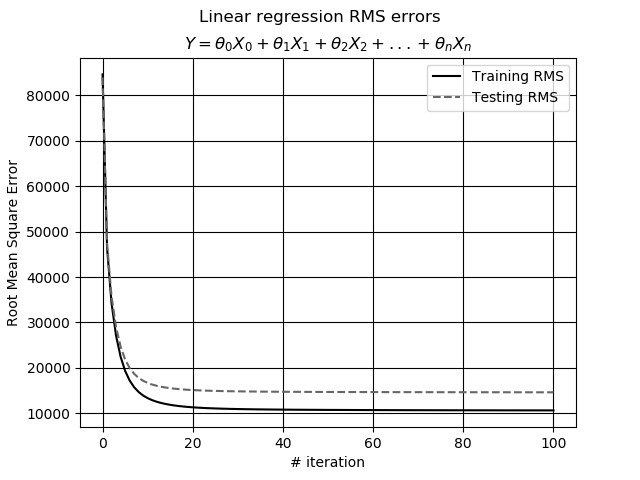
\includegraphics[width=0.9\columnwidth]{img/lr-gd.png}
    \caption{RMS obtidos no treinamento e teste a cada iteração.}
    \label{fig:lr-gd}
\end{figure}

A figura \ref{fig:lr-norm}, por sua vez, representa os resultados encontrados a partir do uso da expressão \ref{norm}. Dois gráficos são mostrados: no primeiro, compara-se os erros obtidos no treinamento e teste para diversos tamanhos de conjuntos de entrada indo de 10000 até 31715, enquanto que no segundo, compara-se os vetores \(\bm{\theta}\) obtidos pelos dois métodos descritos nessa seção. Conforme esperado, o RMS encontrado para o método normal, em torno de 10580, foi inferior aquele encontrado por \textit{gradient descent}. O erro de teste, por sua vez, também ficou em torno de 14570. Observa-se também que algumas diferenças consideráveis entre os vetores \(\bm{\theta}\) sobretudo para os conjuntos de dados com tamanhos intermediários.

\begin{figure}
    \centering
    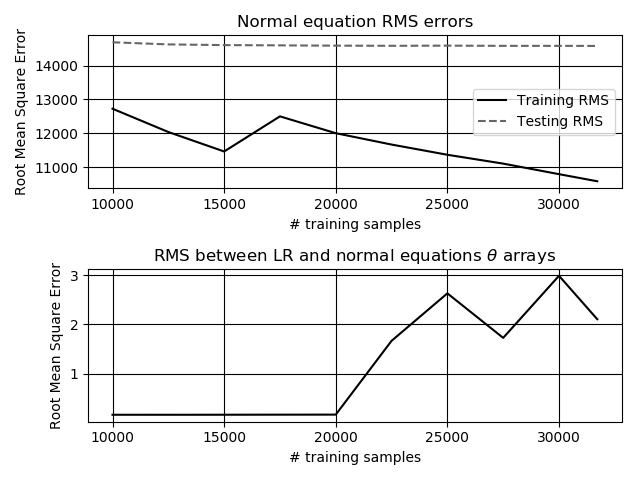
\includegraphics[width=0.9\columnwidth]{img/lr-norm.png}
    \caption{RMS obtidos no treinamento e teste para diversos números de amostras.}
    \label{fig:lr-norm}
\end{figure}

\subsection{Modelo linear simples regularizado}

Apesar de não ter sido observado efeitos de \textit{overfitting} nos resultados anteriores, propomos o uso da regularização, conforme explicado na subseção \ref{sec:reg}. Foram testados dois valores de \(\lambda\), um igual a 1.0 e o outro, vinte vezes maior, 20.0. A figura \ref{fig:reg-comparison} compara os resultados encontrados para a técnica de \textit{gradient descent} entre os modelos regularizados e aquele da subseção anterior. Verifica-se que, para estes casos, a regularização não modificou substantivamente o erro encontrado, tanto para o conjunto de treinamento quanto o de teste. Isso indica que os valores sugeridos de \(\lambda\) são muito pequenos quando comparados a cada um dos fatores \(\bm{\theta}_j^2\) individualmente.  Estes mesmos modelos também foram submetidos às equações normais, porém, assim como no \textit{gradient descent}, nenhuma grande alteração foi observada.

\begin{figure}
    \centering
    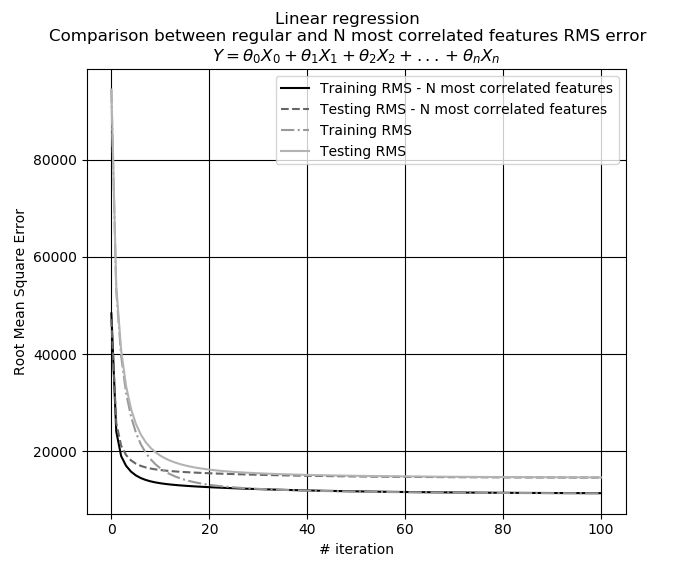
\includegraphics[width=0.9\columnwidth]{img/lr-comparation.png}
    \caption{RMS obtidos nos modelos regularizados.}
    \label{fig:reg-comparison}
\end{figure}

\subsection{Redução de atributos do modelo}

Uma outra tentativa realizada para minimizar o erro foi reduzir o número de atributos utilizados para o modelo. A seleção dos atributos foi feita de acordo com a correlação de cada um deles em relação à saída, uma vez que, como o modelo ainda é linear, espera-se que variáveis mais correlatas sigam o mesmo padrão que aquele observado na saída. A figura \ref {fig:correlation} representa apenas as 10 variáveis mais correlatas e que foram utilizadas para o novo modelo proposto. Vale dizer que a correlação mais alta, correspondente ao atributo 25 (\textit{Avg. keyword (avg. shares)}), ainda é um valor bem baixo, isto é, 0.125, indicando que nenhuma vaiável influencia fortemente o número de compartilhamentos de uma publicação. A figura \ref{fig:comparison-selection} compara os resultados encontrados para o modelo linear simples e para o modelo proposto nesta subseção. Observa-se um ligeiro aumento do erro de treinamento para o modelo reduzido a partir da iteração 10, indicando uma leve presença de \textit {overfitting}. Além disso, verifica-se que ambos os erros de treinamento e teste do modelo reduzido convergem mais rapidamente do que aqueles do modelos simples aos valores onde permanecem praticamente constantes. Por fim, ressalta-se que as equações normais também foram utilizadas, porém seus resultados não são representados neste relatório por efeitos de simplificação.

\begin{figure}
    \centering
    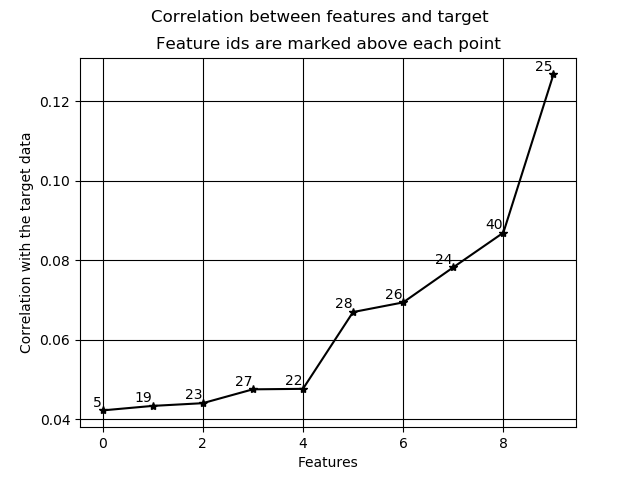
\includegraphics[width=0.9\columnwidth]{img/lr-selection.png}
    \caption{Correlação dos atributos de entrada com a saída.}
    \label{fig:correlation}
\end{figure}

\begin{figure}
    \centering
    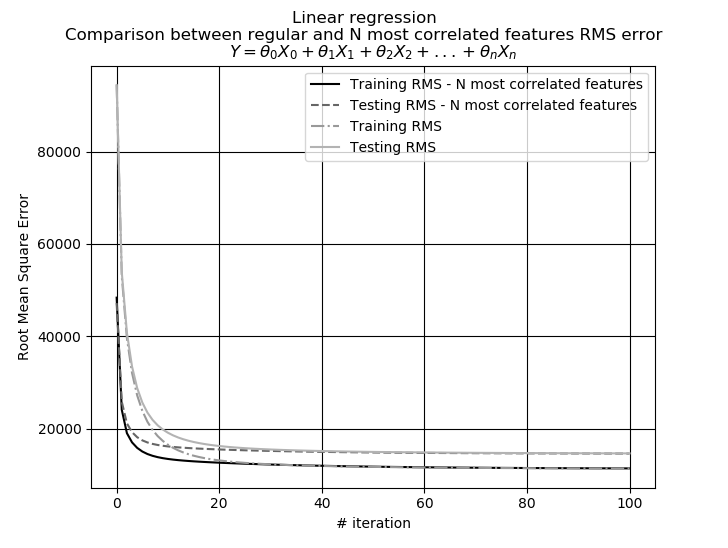
\includegraphics[width=0.9\columnwidth]{img/lr-comparation-selection.png}
    \caption{Comparação entre modelo linear simples e aquele com as 10 variáveis mais correlatas com a saída.}
    \label{fig:comparison-selection}
\end{figure}

\subsection{Modelo linear com atributos de segunda ordem}

Outra técnica que pode ser empregada para reduzir os erros de treinamento e teste é a adição de novos atributos baseados nos já existentes ao modelo simples. Nessa etapa, portanto, adiciona-se ao modelo linear simples todas as suas variáveis ao quadrado, de forma a obter a nova relação \(Y_2 = Y + \theta_{N+1}X_1^2 + \theta_{N+2}X_2^2 + \ldots + \theta_{2N}X_N^2\). Espera-se com esse novo modelo uma melhor adequação aos dados de treinamento e aos de teste simultaneamente, isto é, sem a observação de \textit{overfitting}.  Vale lembrar que as equações \ref{normal} e \ref{gd} não sofrem quaisquer alterações, dado o fato que a equação de custo \ref{cost} continua linear em \(\bm{\theta}\). A figura \ref{fig:gd-second} possui o resultado da técnica de \textit{gradient descent} para este modelo. Observa-se que na iteração 17, o valor de \(\alpha\) é modificado, conforme descrito na seção \ref{sec:ajuste}, uma vez que o erro produzido foi superior àquele encontrado na iteração precedente. Os erros RMS de treinamento e de teste ao fim de 100 iterações encontrados foram, respectivamente, 11830 e 15570, superiores àqueles verificados para o modelo linear simples. O uso da equação \ref{normal}, por sua vez, resultou em erros em torno de 10540 e 14580, muito parecidos àqueles obtidos pela mesma técnica aplicado ao modelo linear simples.

\begin{figure}
    \centering
    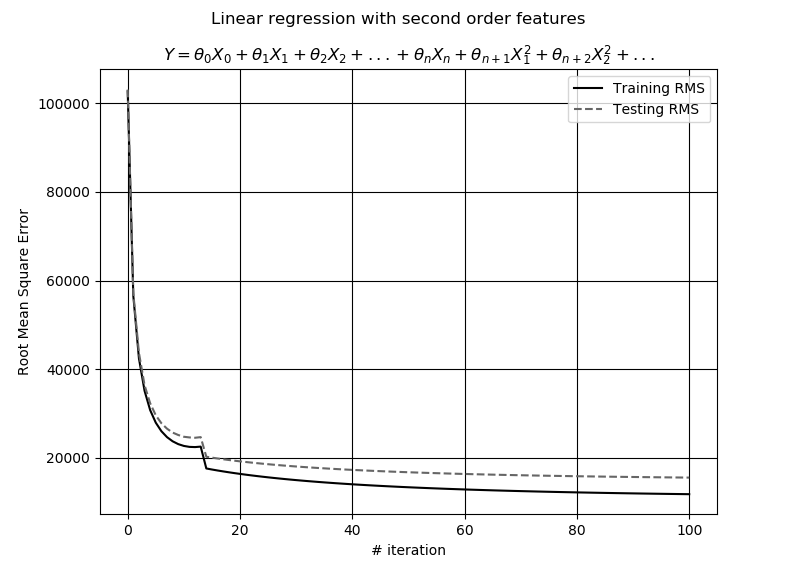
\includegraphics[width=0.9\columnwidth]{img/lr-second-gd.png}
    \caption{RMS obtidos no treinamento e teste do modelo com atributos de segunda ordem a cada iteração.}
    \label{fig:gd-second}
\end{figure}

\subsection{Modelo linear com atributos de terceira ordem}

O último modelo testado neste relatório utilizou atributos de segunda e terceira ordens, obtendo a expressão \(Y_3 = Y_2 + \theta_{2N+1}X_1^3 + \theta_{2N+2}X_2^3 + \ldots + \theta_{3N}X_N^3\). A figura \ref{fig:gd-third} possui a evolução dos erros encontrados no decorrer das 100 iterações. Assim como ocorrido na figura \ref{fig:gd-second}, o valor do parâmetro \(\alpha\) - \textit{learning rate} - teve que ser diminuído, já que o erro de treinamento da iteração 3 foi superior àquele da iteração 2. Os menores erros RMS encontrados para treinamento e teste foram, respectivamente, 12743 e 16208, superiores àqueles obtidos no modelo linear simples. Por fim, o uso das equações normais resultou em erros iguais a 10458 e 15084. O primeiro foi ligeiramente inferior àquele do modelo simples, enquanto que o segundo, superior. Esse fato ilustra bem uma das dificuldades encontradas quando aumenta-se a complexidade do modelo, o \textit{overfitting}. Neste caso, diminui-se o erro do conjunto de treinamento, porém aumenta-se o do conjunto de teste, indicando que o modelo se adequou de maneira exagerada aos dados de treinamento. Conforme já discutido, uma das possíveis soluções a este problema é a regularização.

\begin{figure}
    \centering
    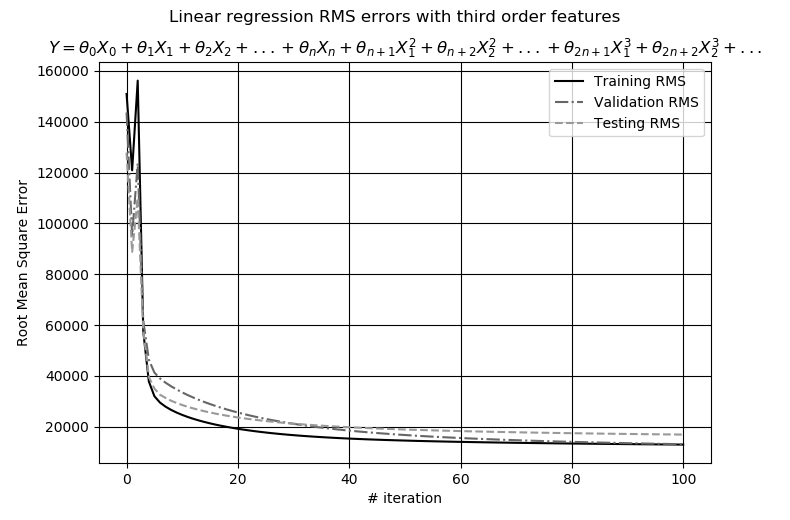
\includegraphics[width=0.9\columnwidth]{img/lr-third-gd.png}
    \caption{RMS obtidos no treinamento e teste do modelo com atributos de segunda e terceira ordens a cada iteração.}
    \label{fig:gd-third}
\end{figure}

%%% Add section %%%%%%%%%%%%%%%%%%%%%%%%%%%%%%%%%%%%%%%%%%%%%%%%%%%%%%%%%%%%%%%%%%
\section{Conclusions}

Cinco modelos lineares foram propostos para a predição do número de compartilhamentos de uma publicação da rede social Mashable. Em praticamente todos eles, os erros RMS de treinamento e teste ficaram em torno de 10500 e 14500, respectivamente, indicando que o modelo linear não é capaz de modelar com precisão o comportamento dos usuários desta rede social.

%%% References %%%%%%%%%%%%%%%%%%%%%%%%%%%%%%%%%%%%%%%%%%%%%%%%%%%%%%%%%%%%%%%%%%%
{\small
\bibliographystyle{unsrt}
\bibliography{refs}
}

\end{document}
